\documentclass[12pt,t]{beamer}

%------------------------------------------------------------------------------
% configuration
%------------------------------------------------------------------------------
\RequirePackage{etex}
\usepackage{textcomp}
\usepackage{../../themes/dbt}
\usepackage{catchfilebetweentags}

\setbeameroption{hide notes}
\setbeamertemplate{caption}{\raggedright\insertcaption\par}

\graphicspath{{images/}}

% a few macros
\newcommand{\bi}{\begin{itemize}}
\newcommand{\ei}{\end{itemize}}
\newcommand{\ig}{\includegraphics}
\newcommand{\src}[2]{\vspace{-10pt}\caption{\href{#1}{\centering \tt \tiny [#2]}}}
\newcommand{\myhref}[1]{\href{#1}{\tt \scriptsize #1}}
\newcommand{\incnote}[1]{\note{\ExecuteMetaData[notes.tex]{#1}}}

%------------------------------------------------------------------------------
% title
%------------------------------------------------------------------------------
% slide
\title{Systèmes d'exploitation pour l'embarqué}
\subtitle{UV 5.2 - Exécution et Concurrence}

\author{\href{}{Paul Blottière}}
\institute{
    \href{http://www.ensta-bretagne.fr/}{ENSTA Bretagne} \\[2pt]
    \href{}{\tt \scriptsize 10 Novembre 2015}
}
\date{
    \href{https://github.com/pblottiere}{\tt \scriptsize https://github.com/pblottiere} \\ [2pt]
    %\href{blottiere.paul@gmail.com}{\tt \scriptsize blottiere.paul@gmail.com}
}

% info
\begin{document}

{
\setbeamertemplate{footline}{} % no page number here
\frame{
    \titlepage
    \incnote{title}
} }

%------------------------------------------------------------------------------
% amélioration continue
%------------------------------------------------------------------------------
\begin{frame}{Amélioration continue}
    \subt{Contributions}
    \vspace{12pt}

    \begin{center}
    
\includegraphics[scale=0.7]{github.png}
    \end{center}

    \bi
    \itemsep12pt
    \item Dépôt du cours : \href{https://github.com/pblottiere/embsys}{\tt \scriptsize https://github.com/pblottiere/embsys}

        \onslide<2->{
            \item Souhaits d'amélioration, erreurs, idées de TP, ... : ouverture d'Issues (avec le bon label!)
            \item Apports de corrections : Pull Request
    }

    \ei
\end{frame}

%------------------------------------------------------------------------------
% organisation
%------------------------------------------------------------------------------
\begin{frame}{Organisation}
    \subt{Volume horaire : 35 heures}
    \vspace{12pt}

    \onslide<2->{
        9 cours :
        \bi
        \itemsep12pt
        \item Introduction, Généralités
        \item Programmation Système
        \item Linux embarqué
        \ei

        \onslide<3->{
            \vspace{12pt}
            Le reste : des travaux pratiques
            \vspace{12pt}
            \bi
            \itemsep12pt
            \item Programmation sous Linux
            \item Utilisation d'outils pour l'embarqué : Armadeus APF28
            \ei
        }
    }

    \incnote{organisation}
\end{frame}

%<**lecture_content>
%------------------------------------------------------------------------------
% lecture
%------------------------------------------------------------------------------
\begin{frame}[plain,c]
    \centering
    \huge\textcolor{title}{Introduction}
\end{frame}

%------------------------------------------------------------------------------
% plan
%------------------------------------------------------------------------------
\begin{frame}{Plan}
    \subt{}

    \begin{enumerate}
        \itemsep4pt
        \item Un peu d'histoire
        \item Les normes
        \item Logiciel Libre et Logiciel Open-Source
        \item Licences de distribution
        \item Définitions et propriétés
        \item Quelques chiffres
        \item Les OS embarqués existants
        \item Comment choisir?
        \item Et si on choisit Linux...
        \item Aspects matériels
        \item Conclusion
        \item Références
        \end{enumerate}

    \note {
    }
\end{frame}

%------------------------------------------------------------------------------
% histoire1
%------------------------------------------------------------------------------
\begin{frame}{Un peu d'histoire (1)}
    \subt{Le premier jeu vidéo}
    \vspace{5pt}

    \onslide<2->{
        \begin{columns}[onlytextwidth]
            \begin{column}{0.45\textwidth}
                \begin{figure}
                    \centering
                    1964 : Multics \\
                    \vspace{30pt}
                    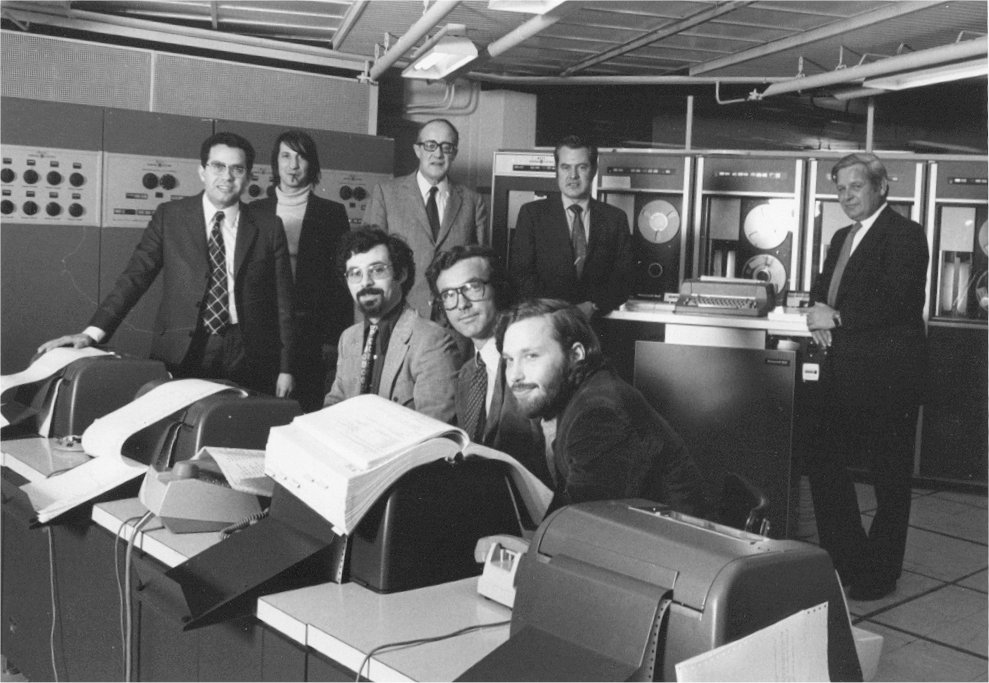
\includegraphics[scale=0.15]{ge645-paris.jpg}
                    \src{http://www.feb-patrimoine.com/projet/multics/multics.htm}{GE-645 - 1972}
                \end{figure}
            \end{column}

            \onslide<3->{
                \begin{column}{0.45\textwidth}
                    \begin{figure}
                        \centering
                        1969 : Space Travel/Unics par Ken Thompson \\
                        \vspace{10pt}
                        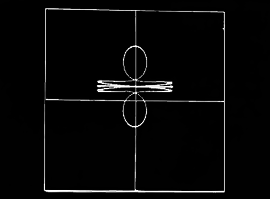
\includegraphics[scale=0.6]{space-travel.png}
                        \src{https://en.wikipedia.org/wiki/Space_Travel_\%28video_game\%29}{Gameplay image of Space Travel}
                    \end{figure}
                \end{column}
            }
        \end{columns}
    }

    \incnote{histoire1}
\end{frame}

%------------------------------------------------------------------------------
% histoire2
%------------------------------------------------------------------------------
\begin{frame}{Un peu d'histoire (2)}
    \subt{La naissance du langage C}

    \onslide<2->{
        \begin{columns}[onlytextwidth]
            \begin{column}{0.45\textwidth}
                \begin{figure}
                    \centering
                    1971 : Le C par Dennis Ritchie \\
                    \vspace{10pt}
                    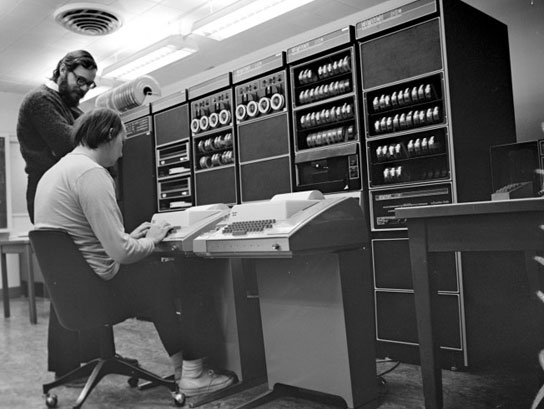
\includegraphics[scale=0.3]{ken-ritchie-1972.jpg}
                    \src{http://www.nextinpact.com/archive/66368-dennis-ritchie-deces-langage-c-unix.htm}{Dennis Ritchie et Kenneth Thompson}
                \end{figure}
            \end{column}

            \onslide<3->{
                \begin{column}{0.45\textwidth}
                    \begin{figure}
                        \centering
                        1983 : GNU par Stallman \\
                        \vspace{10pt}
                        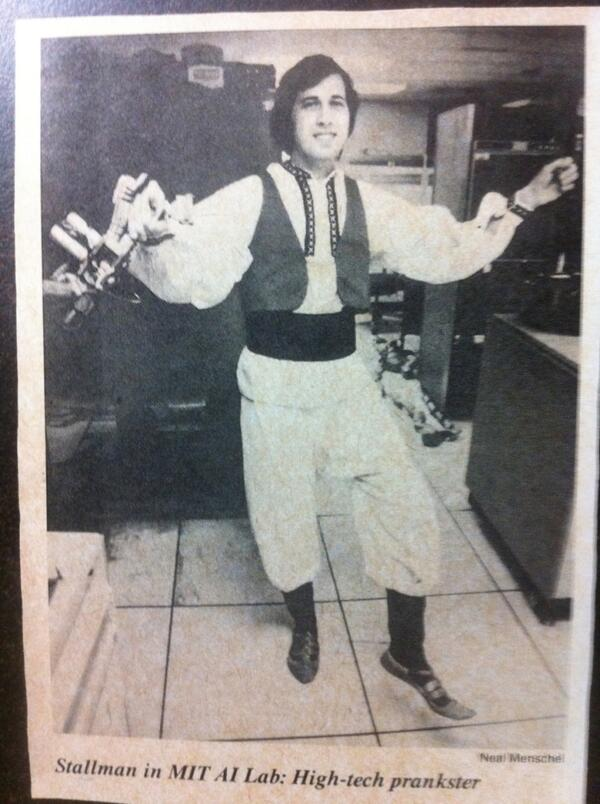
\includegraphics[scale=0.15]{rms-mitlab.jpg}
                        \src{http://ergoemacs.org/misc/Richard_Stallman_at_MIT_dancing.html}{RMS in MIT - pre 1985}
                    \end{figure}
                \end{column}
            }
        \end{columns}
    }

    \incnote{histoire2}
\end{frame}

%------------------------------------------------------------------------------
% histoire3
%------------------------------------------------------------------------------
\begin{frame}{Un peu d'histoire (3)}
    \subt{Un hobby devenu célèbre}
    \vspace{10pt}

    \onslide<2->{
        \begin{columns}[onlytextwidth]
            \begin{column}{0.45\textwidth}
                \begin{figure}
                    \centering
                    1987 : Linux par Linus Torvalds \\
                    \vspace{10pt}
                    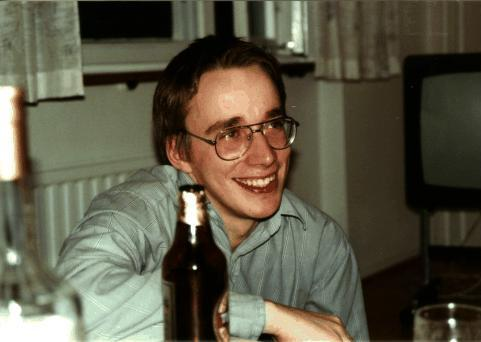
\includegraphics[scale=0.3]{linus.jpg}
                    \src{http://www.linuxfocus.org/common/November1997/linus.gif}{Linus Tovalds}
                \end{figure}
            \end{column}

            \onslide<3->{
                \begin{column}{0.45\textwidth}
                    \begin{figure}
                        \centering
                        1992 : GNU / Linux \\
                        \vspace{30pt}
                        
\includegraphics[scale=0.2]{gnu-linux.png}
                    \end{figure}
                \end{column}
            }
        \end{columns}
    }

    \incnote{histoire3}
\end{frame}

%------------------------------------------------------------------------------
% histoire4
%------------------------------------------------------------------------------
\begin{frame}{Un peu d'histoire (4)}
    \subt{De nos jours}
    \vspace{5pt}

    \begin{figure}
        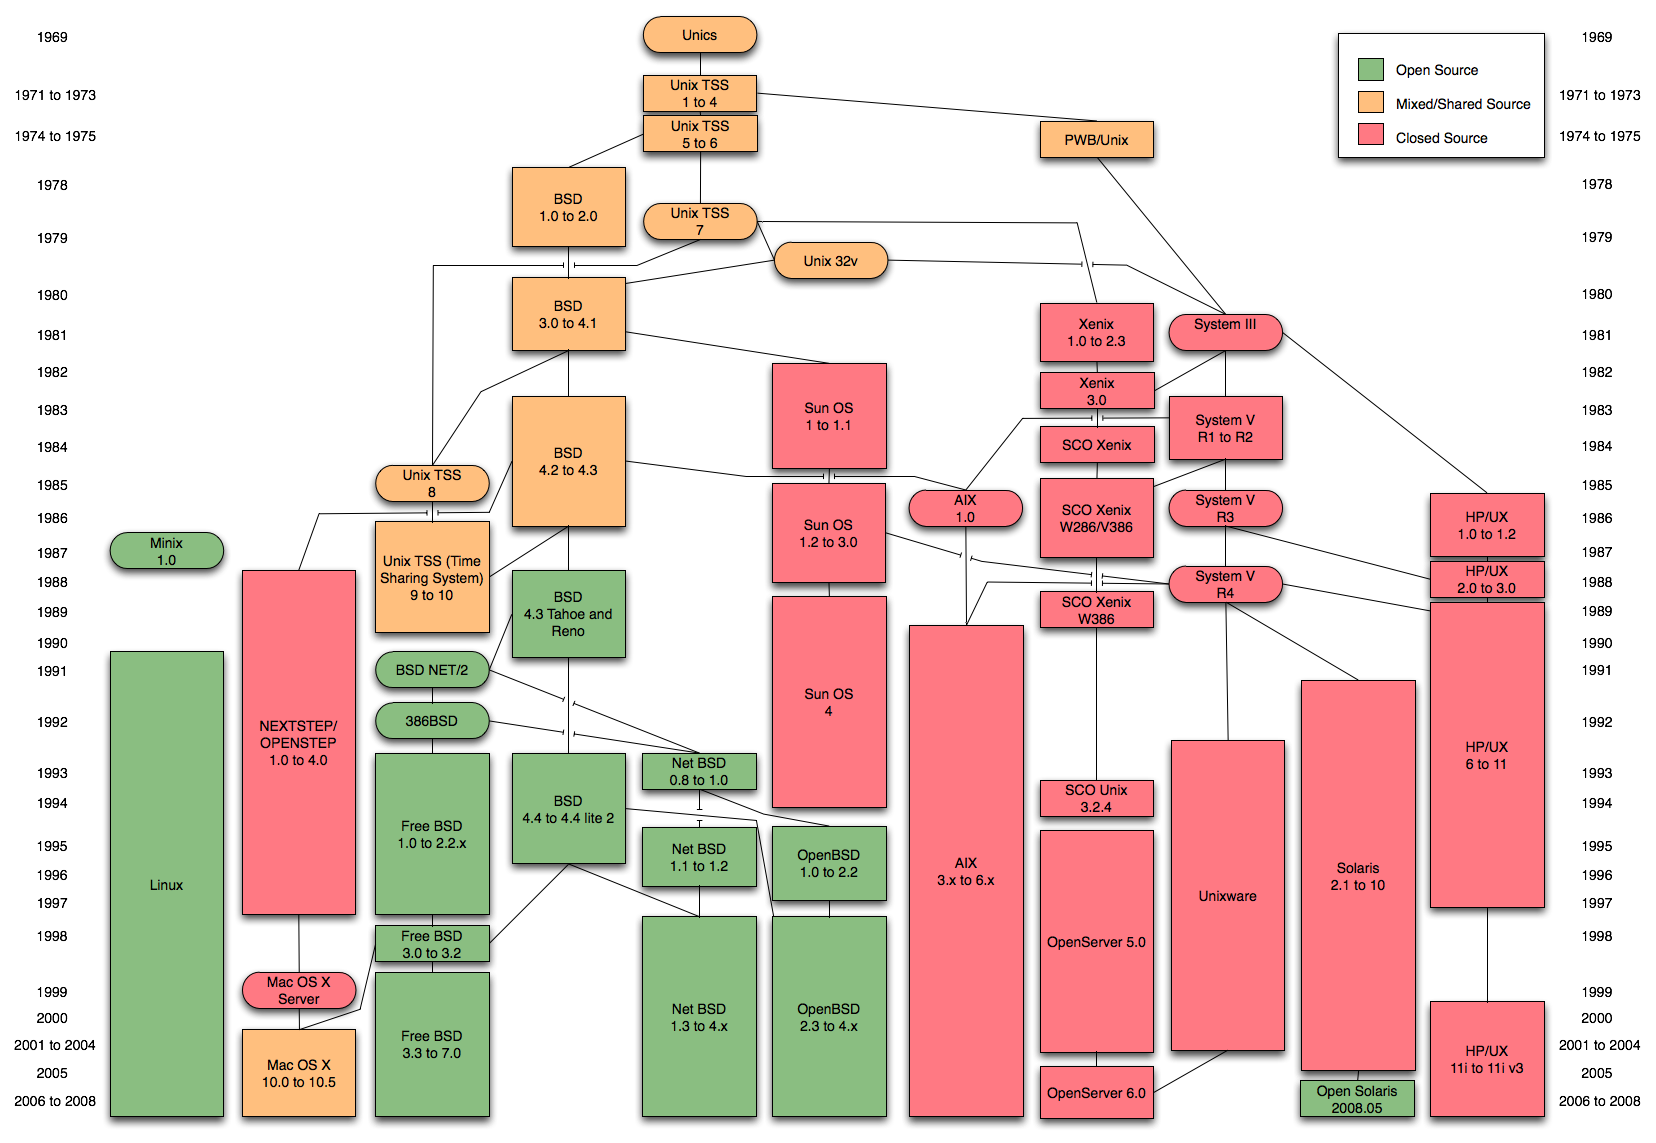
\includegraphics[scale=0.17]{timeline.png}
        \src{https://en.wikipedia.org/wiki/File:Unix_history-simple.svg}{UNIX timeline}
    \end{figure}

    \incnote{histoire4}
\end{frame}

%------------------------------------------------------------------------------
% normes1
%------------------------------------------------------------------------------
\begin{frame}{Les normes (1)}
    \subt{SUSv4}
    \vspace{20pt}

    Des normes sont nécessaires pour assurer une compatibilité des logiciels
    entre systèmes d'exploitation:
    \vspace{10pt}
    \bi
    \itemsep12pt
    \item 1988 : Portable Operating System Interface (POSIX). Plusieurs
          versions : 1, 1.b, 1.c
    \item 1997 : UNIX98 ou Single UNIX Specification V2
    \item Standard actuel : SUSv4 (fusion entre POSIX et UNIX98)
    \ei

    \vspace{10pt}
    \centering
    \myhref{http://www.unix.org/version4/}

    \incnote{normes1}
\end{frame}

%------------------------------------------------------------------------------
% normes2
%------------------------------------------------------------------------------
\defverbatim{\lstposxily}{
    \begin{lstlisting}
    > ls -a .
    .vimrc .vim devel doc
    > ls . -a
    .vimrc .vim devel doc
    > POSIXLY_CORRECT=1 ls . -a
    ls: impossible d'accéder à -a: Aucun fichier ou
        dossier de ce type
    .vimrc .vim devel doc
    \end{lstlisting}
}

\begin{frame}[fragile]{Les normes (2)}
    \subt{POSIXLY\_CORRECT SIR!}
    \vspace{10pt}

    POSIX:
    \begin{lstlisting}[language=bash]
tool [-a][-b][-c option_argument] \
     [-d|-e][-f[option_argument]][operand...]
    \end{lstlisting}

    \vspace{10pt}
    Sous GNU/Linux, les règles sont différentes!

    \onslide<2->{
        \vspace{10pt}
        Conséquences sous une distribution Linux:

        \lstposxily
    }

    \incnote{normes2}
\end{frame}

%------------------------------------------------------------------------------
% opensource1
%------------------------------------------------------------------------------
\begin{frame}{Logiciel Libre et Logiciel Open Source (1)}
    \subt{Question de philosophie...}
    \vspace{20pt}

    \bi
    \item Logiciel Libre : code source ouvert et pouvant être modifié. Fond
        philosophique => liberté des utilisateurs (Free as Freedom)!
    \vspace{20pt}

    \onslide<2->{
        \item Logiciel Open Source : code source ouvert et pouvant être modifié...
              Fond pragmatique => efficacité, praticité!
    \ei
    }

    \onslide<3->{
        \vspace{10pt}
        \centering
        \myhref{http://www.gnu.org/philosophy/free-software-for-freedom.fr.html}
    }

    \incnote {opensource1}
\end{frame}

%------------------------------------------------------------------------------
% opensource2
%------------------------------------------------------------------------------
\begin{frame}{Logiciel Libre et Logiciel Open Source (2)}
    \subt{Origine des licences GPL et LGPL}
    \vspace{15pt}

    \vspace{5pt}
    \begin{center}
    1985 \\
    \vspace{10pt}
    
\includegraphics[scale=0.5]{fsf.png}
    \end{center}
    \vspace{5pt}

    \onslide<2->{
        Son but:
        \bi
        \itemsep12pt
        \item protéger les utilisateurs contre les logiciels "privateurs"
        \item élaborer des licences de distribution
        \ei
    }

    \incnote{opensource2}
\end{frame}

%------------------------------------------------------------------------------
% licences1
%------------------------------------------------------------------------------
\begin{frame}{Licences de distribution (1)}
    \subt{Copyleft}
    \vspace{20pt}

    L'utilisateur refuse qu'une évolution quelconque de son travail soit
    accompagnée d'une restriction!

    \vspace{40pt}
    \centering
    
\includegraphics[scale=0.25]{copyleft.png}

    \incnote {licences1}
\end{frame}

%------------------------------------------------------------------------------
% licences2
%------------------------------------------------------------------------------
\begin{frame}{Licences de distribution (2)}
    \subt{GPL et LGPL}
    \vspace{20pt}

    Licence libre copyleft :
    \bi
    \item GPL : GNU General Public Licence. Édition de liens possible qu'avec du
          code GPL! \myhref{http://www.gnu.org/licenses/gpl-3.0.fr.html}
    \item LGPL : Lesser GPL. Édition de liens moins restrictive! \myhref{http://www.gnu.org/licenses/lgpl-3.0.fr.html}
    \ei

    \onslide<2->{
        \vspace{20pt}
        Licence libre non copyleft :
        \bi
        \item BSD : les versions modifiées ne sont elles mêmes pas nécessairement
              libres!
        \item ...
        \ei
    }

    \incnote {licences2}
\end{frame}

%------------------------------------------------------------------------------
% licences3
%------------------------------------------------------------------------------
\begin{frame}[fragile]{Licences de distribution (3)}
    \subt{Conséquences dans la vie courante...}
    \vspace{15pt}

    Examples de licences:
    \bi
    \itemsep6pt
    \item nmap : GPL {\tt /usr/share/doc/nmap/copyright}
    \item GNU C library : LGPL {\tt /usr/share/doc/libc6/copyright}
    \ei
    \vspace{20pt}

    \onslide<2->{
        Debian et le DFSG (Debian Free Software Guideline) :
        \bi
        \item {\tt main} : paquets conforme au DFSG
        \item {\tt contrib} : paquets conforme au DFSG mais avec des dépendances en
            dehors du {\tt main}
        \item {\tt non-free} : paquets non conforme au DFSG
        \ei
    }

    \incnote{licences3}
\end{frame}

%------------------------------------------------------------------------------
% licences4
%------------------------------------------------------------------------------
\begin{frame}[fragile]{Licences de distribution (4)}
    \subt{Conséquences dans la vie courante...}
    \vspace{10pt}

    VRMS (Virtual RMS) :
    \vspace{10pt}
    \begin{lstlisting}
> vrms
Contrib packages installed on multi
flashplugin-nonfree            Adobe Flash Player
1 contrib packages, 0.0% of 2877 installed packages
    \end{lstlisting}

    \begin{figure}
        \centering
        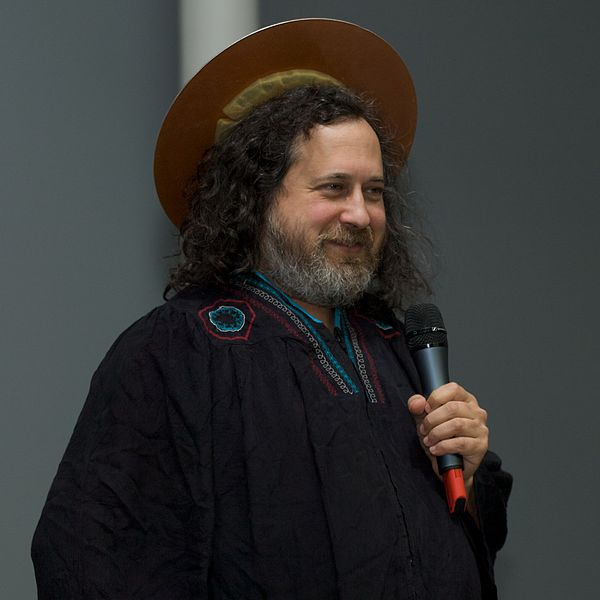
\includegraphics[scale=0.15]{ignucius.jpg}
        \src{https://commons.wikimedia.org/wiki/File:NicoBZH_-_Richard_Stallman_\%28by-sa\%29_\%288\%29.jpg}{RMS : Saint Ignucius}
    \end{figure}

\end{frame}

%------------------------------------------------------------------------------
% def1
%------------------------------------------------------------------------------
\begin{frame}{Définitions et propriétés (1)}
    \subt{Kernel et système d'exploitation}
    \vspace{10pt}

    Kernel :
    \bi
    \item noyau d'un système d'exploitation
    \item gère les ressources matérielles
    \item permet la communication entre composants logiciels/matériels
    \item existe plusieurs architectures (voir cours suivant)
    \ei

    \onslide<2->{
        \vspace{10pt}
        Système d'exploitation:
        \bi
        \item kernel + logiciels comme compilateur, shell, debuger, ...
        \item couche d'abstraction par rapport au matériel
        \item interface générique de programmation
        \ei
    }

    \incnote{def1}
\end{frame}

%------------------------------------------------------------------------------
% def2
%------------------------------------------------------------------------------
\begin{frame}{Définitions et propriétés (2)}
    \subt{Dans le monde des systèmes embarqués...}
    \vspace{5pt}

    Système embarqué:
    \bi
    \itemsep4pt
    \item composition d'une partie électronique et logicielle
    \item souvent très limitée d'un point de vue ressources matérielles (CPU,
          mémoire, ...)
    \item autonome, durée de vie très longue (plus de 20 ans pour les systèmes
          militaires)
    \item doit respecter des contraintes d'environnement (vibration, chaleur,
          ...)
    \ei

    \vspace{5pt}
    \centering
    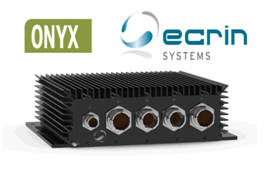
\includegraphics[scale=0.5]{onyx.png}

    \incnote{def2}
\end{frame}

%------------------------------------------------------------------------------
% def3
%------------------------------------------------------------------------------
\begin{frame}{Définitions et propriétés (3)}
    \subt{Dans le monde des systèmes embarqués}
    \vspace{20pt}

    Système d'exploitation embarqué:
    \bi
    \itemsep6pt
    \item OS sur lequel un logiciel embarqué va être exécuté.
    \item Contrainte forte par rapport à la consommation matérielle /
          énergétique.
    \item OS classique souvent inenvisageable
    \ei
    \vspace{10pt}

    \onslide<2->{
        Système d'exploitation temps réel (vs temps partagé):
        \bi
        \itemsep6pt
        \item garantit les temps de réponse (temps réel dur/mou, préemptivité du
              Kernel, ...)
        \item Voir le cours associé!
        \ei
    }

    \incnote{def3}
\end{frame}

%------------------------------------------------------------------------------
% def4
%------------------------------------------------------------------------------
\begin{frame}{Définitions et propriétés (4)}
    \subt{Dans le monde des systèmes embarqués}
    \vspace{10pt}

    Logiciel embarqué:
    \bi
    \itemsep6pt
    \item logiciel intégré pour une application dédiée
    \item un bon logiciel embarqué est un logiciel dont on oubli l'existence!
    \ei

    \onslide<2->{
        \vspace{10pt}
        Linux embarqué
        \bi
        \itemsep6pt
        \item Kernel Linux + composants open-source
        \item construit sur mesure par rapport aux besoins
        \ei

        \vspace{10pt}
        \centering
        
\includegraphics[scale=0.8]{linux-embedded.png}
    }

    \incnote{def4}
\end{frame}

%------------------------------------------------------------------------------
% def5
%------------------------------------------------------------------------------
\begin{frame}{Définitions et propriétés (5)}
    \subt{Rappels : microcontrôlleur vs microprocesseur}
    \vspace{10pt}

    Microprocesseur:
    \bi
    \itemsep6pt
    \item séquenceur
    \item unité arithmétique et logique (UAL)
    \item registre
    \item unité d'entrée sortie (analogique)
    \ei

    \onslide<2->{
        \vspace{10pt}
        Microcontrôlleur:
        \bi
        \itemsep6pt
        \item microprocesseur peu puissant (fréquence d'horloge faible, largeur des
              registres restreinte : 4 bits/8bits contre 32 bits/64bits, ...)
        \item mémoire intégrée
        \item entrées/sorties analogiques et numériques
        \ei
    }

    \incnote{def4}
\end{frame}

%------------------------------------------------------------------------------
% chiffres1
%------------------------------------------------------------------------------
\begin{frame}{Quelques chiffres (1)}
    \subt{Les systèmes embarqués sont partout!}

    \begin{figure}
        \centering
        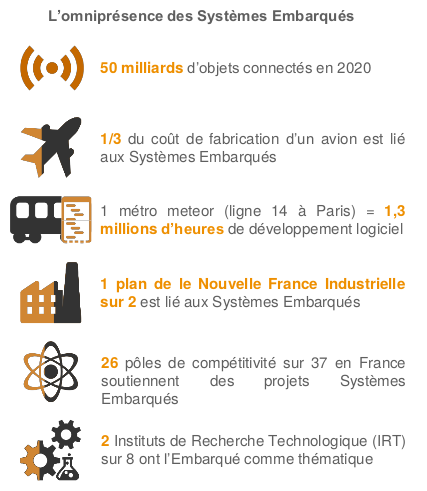
\includegraphics[scale=0.5]{chiffres1.png}
        \src{http://www.fafiec.fr/images/contenu/menuhaut/observatoire/etudes/2013/systemes-embarqu\%C3\%A9s/SE_Synthese_globale_-_20140606.pdf}{OPIIEC - 2014}
    \end{figure}

    \incnote{chiffres1}
\end{frame}

%------------------------------------------------------------------------------
% chiffres2
%------------------------------------------------------------------------------
\begin{frame}{Quelques chiffres (2)}
    \subt{Soutien des états}

    \begin{figure}
        \centering
        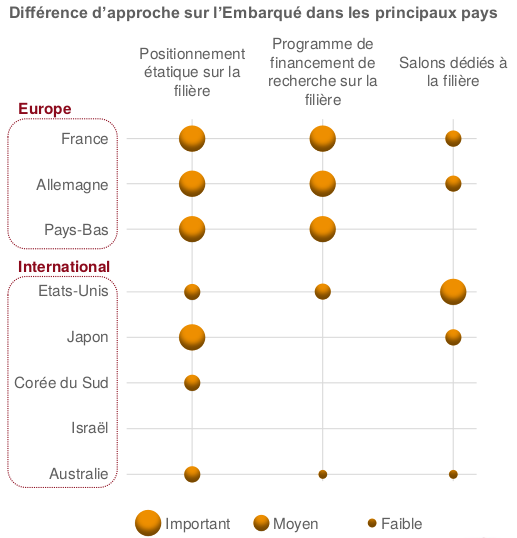
\includegraphics[scale=0.4]{chiffres2.png}
        \src{http://www.fafiec.fr/images/contenu/menuhaut/observatoire/etudes/2013/systemes-embarqu\%C3\%A9s/SE_Synthese_globale_-_20140606.pdf}{OPIIEC - 2014}
    \end{figure}

    \incnote{chiffres2}
\end{frame}

%------------------------------------------------------------------------------
% chiffres3
%------------------------------------------------------------------------------
\begin{frame}{Quelques chiffres (3)}
    \subt{Répartition du Chiffre d'Affaires}

    \vspace{20pt}
    \begin{figure}
        \centering
        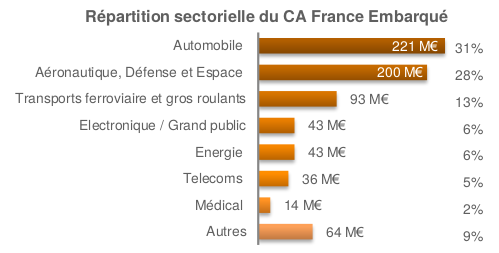
\includegraphics[scale=0.6]{chiffres3.png}
        \src{http://www.fafiec.fr/images/contenu/menuhaut/observatoire/etudes/2013/systemes-embarqu\%C3\%A9s/SE_Synthese_globale_-_20140606.pdf}{OPIIEC - 2014}
    \end{figure}

    \incnote{chiffres3}
\end{frame}

%------------------------------------------------------------------------------
% chiffres4
%------------------------------------------------------------------------------
\begin{frame}{Quelques chiffres (4)}
    \subt{Répartition des effectifs}

    \begin{figure}
        \centering
        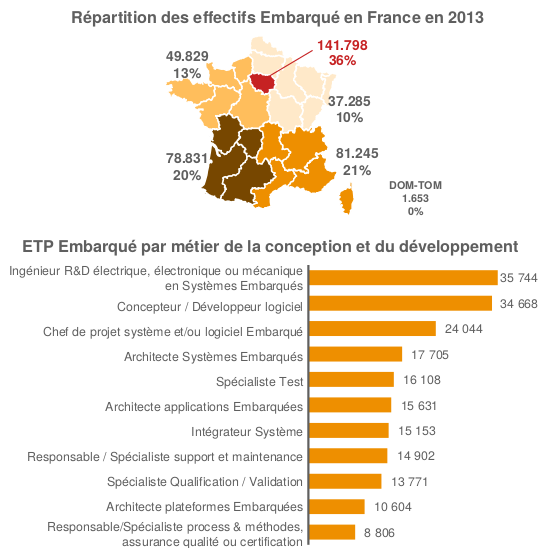
\includegraphics[scale=0.45]{chiffres4.png}
        \src{http://www.fafiec.fr/images/contenu/menuhaut/observatoire/etudes/2013/systemes-embarqu\%C3\%A9s/SE_Synthese_globale_-_20140606.pdf}{OPIIEC - 2014}
    \end{figure}

    \incnote{chiffres4}
\end{frame}

%------------------------------------------------------------------------------
% embos1
%------------------------------------------------------------------------------
\begin{frame}{Les OS embarqués existants (1)}
    \subt{Sans base Linux}
    \vspace{15pt}

    \bi
    \itemsep12pt
    \item VxWorks : noyau temps réel le plus utilisé dans l'industrie. Licence
          très coûteuse!
    \item QNX : npyau temps réel. Gratuit pour les applications non commerciales.
    \item micro-C OS : temps réel pour micro contrôlleur. Gratuit pour
          l'enseignement.
    \item Windows Phone : pour mobile. Se veut concurrent de Android.
    \item Plein d'autres : LunxOS, Nucleus, eCos, ...
    \ei

    \incnote{embos1}
\end{frame}

%------------------------------------------------------------------------------
% embos2
%------------------------------------------------------------------------------
\begin{frame}{Les OS embarqués existants (2)}
    \subt{À base de Linux}

    \vspace{12pt}
    \bi
    \itemsep10pt
    \item Wind River Linux : avec extension temps réel RTLinux
    \item ELDK (Embedded Linux Development Kit) : Fournit une ditribution
          complète pour les architectures PowerPC, ARM et MIPS. Sous licence GPL.
    \item Google Android : application en Java. Existe un SDK C/C++.
    \item Tizen : dernier né (2012), Open Source. OS de la Samsung Gear S2!
    \item Plein d'autres : MontaVista Linux, BlueCat Linux, ...
    \ei

    \incnote{embos2}
\end{frame}

%------------------------------------------------------------------------------
% embos3
%------------------------------------------------------------------------------
\begin{frame}{Les OS embarqués existants (3)}
    \subt{Exemples}

    \begin{columns}[onlytextwidth]
        \begin{column}{0.45\textwidth}
            \begin{figure}
                \centering
                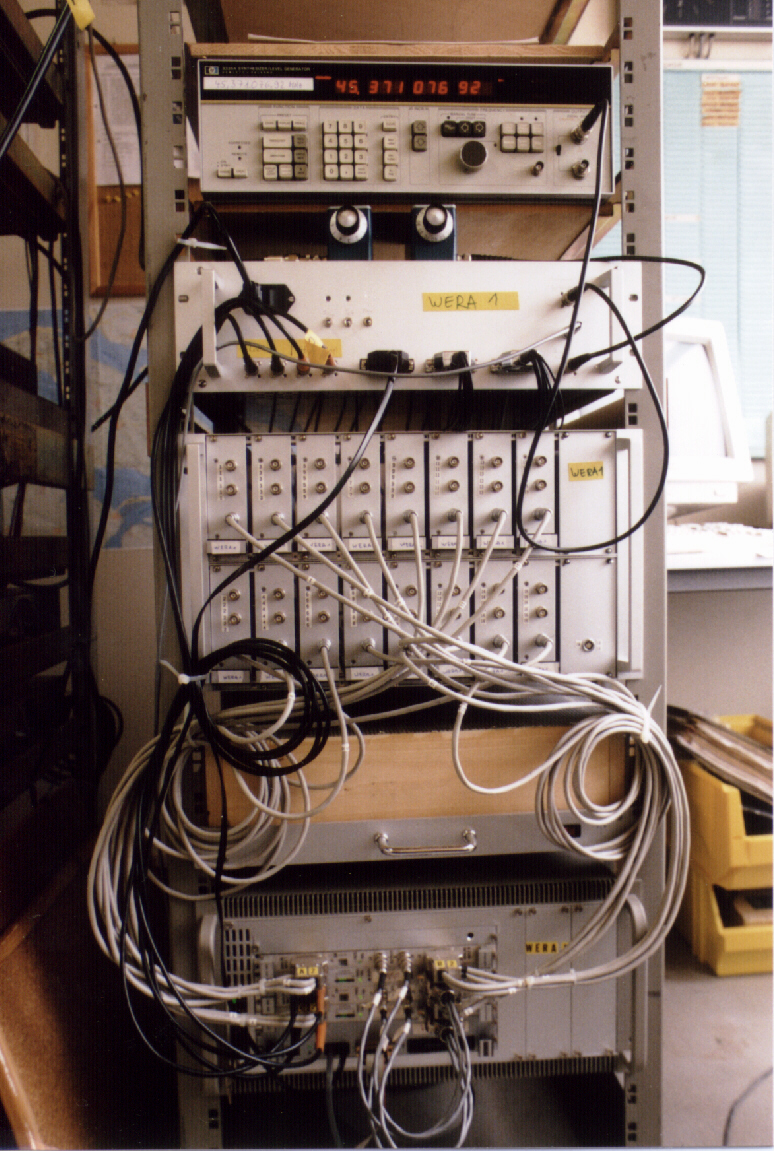
\includegraphics[scale=0.12]{wera.jpg}
                \src{http://ifmaxp1.ifm.uni-hamburg.de/WERA_SYSTEM.JPG}{Radars HF Wera déployés sur les côtes Bretonnes : VxWorks}
            \end{figure}
        \end{column}
        \begin{column}{0.45\textwidth}
            \begin{figure}
                \centering
                \vspace{15pt}
                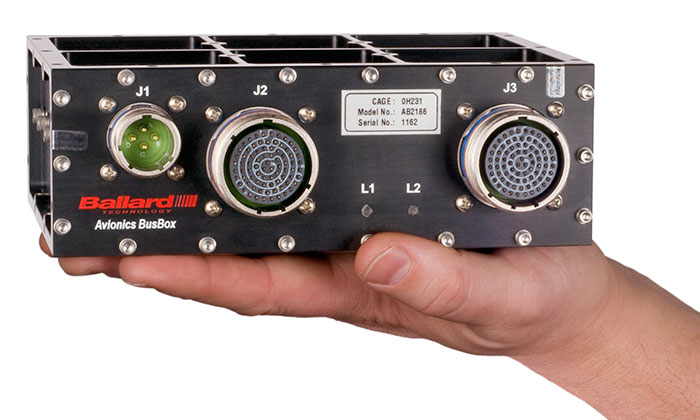
\includegraphics[scale=0.18]{ab2000.jpg}
                \src{http://www.ballardtech.com/products.aspx/dir/category/Embedded_Computers?s=menu}{OmniBusBox Ballard technology : ELDK}
        \end{figure}
        \end{column}
    \end{columns}

\end{frame}

%------------------------------------------------------------------------------
% choice1
%------------------------------------------------------------------------------
\begin{frame}{Comment choisir?! (1)}
    \subt{Systèmes propriétaires ?}
    \vspace{8pt}

    Avantages et inconvénients:
    \bi
    \itemsep6pt
    \item Pas d'effet de masse donc cher (et cher donc pas d'effet de masse...)
    \item Personne maîtrisant les outils associés rares sur le marché de
          l'emploi : rare donc cher!
    \item La durée de vie d'un système embarqué est très élevée. Donc que se
          passe-t-il si l'entreprise propriétaire disparaît? Risqué...
    \item Mais en théorie, très bon support, très bonne réactivité!
    \item Garantie en cas de problème, responsabilité de l'entreprise!
    \ei

    \incnote{choice1}
\end{frame}

%------------------------------------------------------------------------------
% choice2
%------------------------------------------------------------------------------
\begin{frame}{Comment choisir?! (2)}
    \subt{Systèmes Open Source?}
    \vspace{15pt}

    Avantages et inconvénients:
    \bi
    \itemsep12pt
    \item Redistribution sans royalties
    \item Code source ouvert et donc modifiable à volonté! Mais les licences
          trop ouverte (comme la GPL) peutvent poser problèmes pour les
          entrerpises ne souhaitant pas reverser leurs travaux!
    \item Logiciel fourni "As is". Problème de responsabilité?
    \item Argument non nécessairement objectif : code souvent de bien meilleur
          qualité!
    \ei

    \incnote{choice2}
\end{frame}

%------------------------------------------------------------------------------
% linux1
%------------------------------------------------------------------------------
\begin{frame}{Et si on choisit Linux... (1)}
    \subt{Avantages}

    Reconnu pour sa très grande fiabilité!
    \begin{figure}
        \centering
        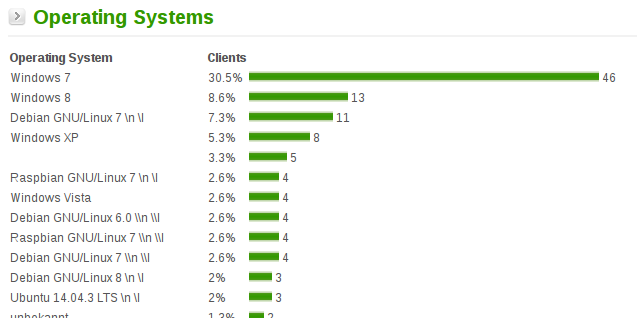
\includegraphics[scale=0.3]{uptime_os.png}
        \src{http://en.uptime24.net/stats.php}{Uptime project - Operating System statistics - 2015}
    \end{figure}

    \begin{figure}
        \centering
        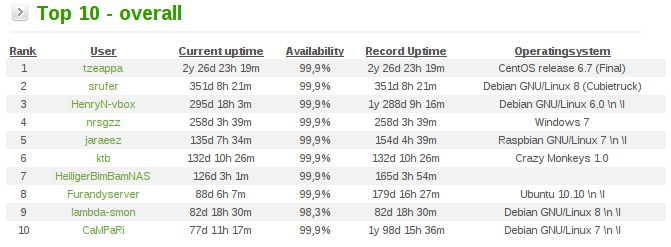
\includegraphics[scale=0.4]{uptime.png}
        \src{http://en.uptime24.net/toplist.php?do=top10}{Uptime project - top 10 - 2015}
    \end{figure}

\incnote{linux1}
\end{frame}

%------------------------------------------------------------------------------
% linux2
%------------------------------------------------------------------------------
\begin{frame}{Et si on choisit Linux... (2)}
    \subt{Avantages}
    \vspace{20pt}

    Comme vu dans les parties précédentes:
    \vspace{10pt}
    \bi
    \itemsep12pt
    \item Peu cher : pas de royalties, outils de développement libres, ...
    \item Portabilté : x86, arm, ppc, amd, sparc, ...
    \item Open Source
    \ei

    \incnote{linux2}
\end{frame}

%------------------------------------------------------------------------------
% linux3
%------------------------------------------------------------------------------
\begin{frame}{Et si on choisit Linux... (3)}
    \subt{Inconvénients}

    \vspace{10pt}
    \bi
    \itemsep12pt
    \item Beaucoup de licences. Plus compliqué qu'une seule licence propriétaire.
    \item Beaucoup de solutions pour faire la même chose contrairement à une
          solution propriétaire sur étagère.
    \ei

    \begin{figure}
        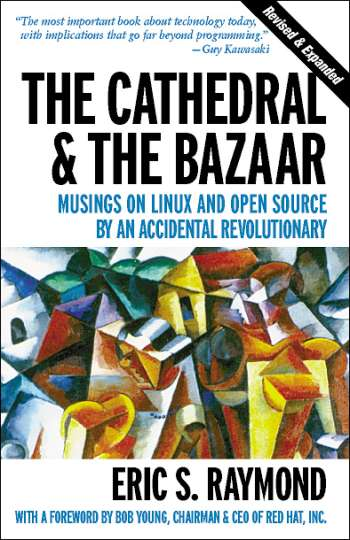
\includegraphics[scale=0.2]{bazaar.jpg}
        \src{http://www.seattlestar.net/2013/12/the-cathedral-and-the-bazaar/}{The Cathedral and the bazaar}
    \end{figure}

    \incnote{linux3}
\end{frame}

%------------------------------------------------------------------------------
% hard1
%------------------------------------------------------------------------------
\begin{frame}{Aspects matériels (1)}
    \subt{Processeurs}

    \vspace{15pt}
    Le kernel Linux tourne sur de très nombreuses architectures de processeurs
    32 bits et 64 bits.

    \begin{columns}[onlytextwidth]
        \begin{column}{0.45\textwidth}
            \begin{figure}
                \centering
                \vspace{10pt}
                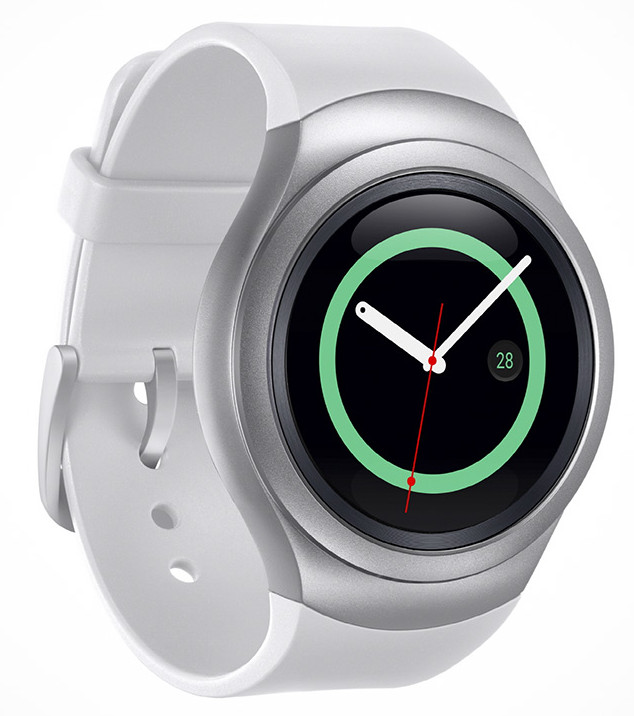
\includegraphics[scale=0.15]{s2.jpg}
                \src{http://www.leblogdomotique.fr/wearable/gear-s2-samsung-tizen-3730}{Samsung Gear S2 - Tizen}
            \end{figure}
        \end{column}
        \begin{column}{0.45\textwidth}
            \begin{figure}
                \centering
                \vspace{10pt}
                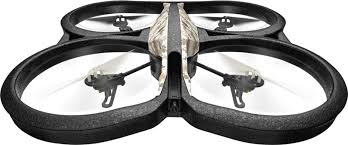
\includegraphics[scale=0.4]{parrot.jpeg}
                \src{http://ardrone2.parrot.com/}{ARDRONE 2.0 - Linux 2.6.32 - Parrot}
            \end{figure}
        \end{column}
    \end{columns}

    \incnote{hard1}
\end{frame}

%------------------------------------------------------------------------------
% hard2
%------------------------------------------------------------------------------
\begin{frame}{Aspects matériels (2)}
    \subt{MMU}

    \vspace{15pt}
    Memory Management Unit (unité de gestion de mémoire) permet de :
    \vspace{10pt}
    \bi
    \itemsep10pt
    \item protéger l'espace mémoire des processus (segmentation fault)
    \item traduction entre adresses physiques et adresses virtuelles
    \ei

    \vspace{15pt}
    Kernel version 2.5.46 : processeurs sans MMU supportés via la \textmu Clibc

    \incnote{hard2}
\end{frame}

%------------------------------------------------------------------------------
% conclusion
%------------------------------------------------------------------------------
\begin{frame}{Conclusion}
    \centering
    \vspace{20pt}
    \huge{Linux, c'est bien!}
    \vspace{15pt}
    \begin{figure}
        
\includegraphics[scale=0.15]{distrib.jpeg}
        \src{http://www.lolita.pf/spip/?lang=fr}{Distributions}
    \end{figure}
\end{frame}

%------------------------------------------------------------------------------
% ref
%------------------------------------------------------------------------------
\begin{frame}{Références}
    \vspace{30pt}

    \bi
    \itemsep12pt
    \item Linux Embarqué - Pierre Ficheux
    \item Développement système sous Linux - Christophe Blaess
    \item Modern Operating Systems - Andrew Tanenbaum
    \ei
\end{frame}
%<//lecture_content>

\end{document}
